     \chapter{Zusammenfassung und Ausblick}
In diesem Projekt handelt es sich um eine Anwendung, die au�ergew�hnliche Situationen mit Hilfe einer Videokamera erkennen kann. Die Applikation orientiert sich an alten Menschen, die allein wohnen. Das Projekt ist eine Kombination von Hintergrundsubtraktion, Histogrammanalyse und Fuzzylogik. Im Rahmen dieser Arbeit wird ein Programm entwickelt, deren Eingaben die Bilder von einer 360� Kamera sind. Das Programm mit Hilfe von der Kamera beobachtet die Person im Alltag und gibt automatisch eine Meldung aus, wenn ein Unfall passiert.\\

Ziel dieses Projekt ist die Entwicklung eine Anwendung, das Videos einer 360� Kamera von Bosch verarbeitet. Das Programm soll eine Bewegung von einer Person erkennen, analysiert und Informationen geben, ob die Person in einer au�ergew�hnlichen Situation ist. Um eine abnormale Situation handelt es sich beispielsweise, wenn eine Person f�r l�ngere Zeit an einem Ort liegt. Um dieses Ziel zu realisieren, wurde das Programm aus drei gro�en Meilensteinen gebaut (Abbildung \ref{fig:zusammenfassung}).
\begin{itemize}
	\item Der erste Meilenstein ist die Hintergrundsubtraktion. In diesem Schritt wird ein Bild als die Eingabe mit einem Hintergrundbild verglichen. Der Unterschied zwischen Eingabebild und Hintergrundbild wird zuerst berechnet und ein Bin�rbild des Vordergrundes wird danach zur�ckgeliefert. Das Bin�rbild stellt eine Silhouette der Person ohne den Hintergrund dar. Das normale Hintergrundsubtraktion-Verfahren hat einen Nachteil, wenn die Person lange sich nicht mehr bewegt, wird die Person in das Hintergrund integriert. Deswegen kann diese Anwendung nicht mehr erkennen, wenn die Person nach einem Unfall sich nicht mehr bewegt. Eine eigene Methode wird in diesem Projekt entwickelt. Die Methode aktualisiert nicht das ganze Hintergrundbild, sondern nur die Begrenzungsboxen, die vergangene Silhouetten enthalten, auf dem Hintergrundbild werden aktualisiert. Diese Methode ist \glqq{}Aktualisierung der selektiven Begrenzungsboxen\grqq{} (ASB) genannt. Obwohl diese Methode eine nicht bewegende Person erkennen kann, ergibt sich das Bin�rbild dieser Methode einige Rauschen.	Eine eigene Methode der Hintergrundsubtraktion wird erweitert. Diese Erweiterung ist eine Kombination von der ASB-Methode und der KNN-Methode in der Arbeit \cite{zivkovic2006efficient} von Zivkovic. Diese Erweiterung ist \glqq{}KNN-Plus-ASB\grqq{} genannt. Bei Aktualisierung des Hintergrundmodells wird das Unterbild des Hintergrundbildes, auf dem es eine Bewegung gibt, nicht betrachtet. Diese Methode kann eine Person erkennen, obwohl die Person sich nicht in der Szene weiter bewegt. Zum Vergleichen mit der ASB-Methode liefert KNN-Plus-ASB bessere Silhouetten in dieser Anwendungsfall. 
	\item In dem zweiten Schritt wird die beschr�nkte Silhouette von dem letzten Schritt weiter analysiert, um die K�rperhaltung der Person zu erkennen. Die Silhouette wird zuerst von der Breite oder H�he auf 128 Pixel skaliert. Aus dem skalierten Bild werden vertikale und horizontale Histogramme gerechnet. Die Histogramme werden weiter mit Referenz-Histogrammen, die aus 4500 Silhouetten von 7 verschiedenen Personen mit 4 K�rperhaltungen (Liegen, Stehen, Beugen, Sitzen) berechnet wurden \cite{haritaoglu1998ghost}, verglichen. Nach dem Vergleichen wird die K�rperhaltung mit  einem maximalen Wert von Loglikelihood-Funktion ausgewertet.
	\item In letztem Schritt wird eine Fuzzylogik angewendet. Diese Methode berechnet einfach wie hoch die Wahrscheinlichkeit ist, dass eine Person unter bestimmten Bedingungen in einer abnormalen Situation ist. Mit Hilfe von der Begrenzungsbox der Silhouette wird ein \inlinecode{C++}{Person}-Objekt aufgebaut, damit die Kamera die gleiche Person in der Szene folgen kann. Die Bedingung f�r einen abnormalen Fall ist: Wenn eine Person auf dem Boden in einem vordefinierten Zeitraum (f�r Testen sind 30 Bildern genommen, aber das Parameter kann f�r spezielle F�lle modifiziert werden) liegt und sich nicht mehr bewegt.
\end{itemize}
Ein Feature der Bosch-360-Grad Kamera ist die F�higkeit, in die Richtigen der Bewegung zu orientieren. Nach der Drehung der Kamera wird das ganze Hintergrundmodell neu aktualisiert, um die Erkennung der Bewegung durch die Hintergrundsubtraktion richtig zu machen. Dies liefert nach Rotation des Kamerakopfes gleichbleibende Ergebnisse wie beim Stillstand der Kamera.\\
\begin{figure}[H]
	\centering
	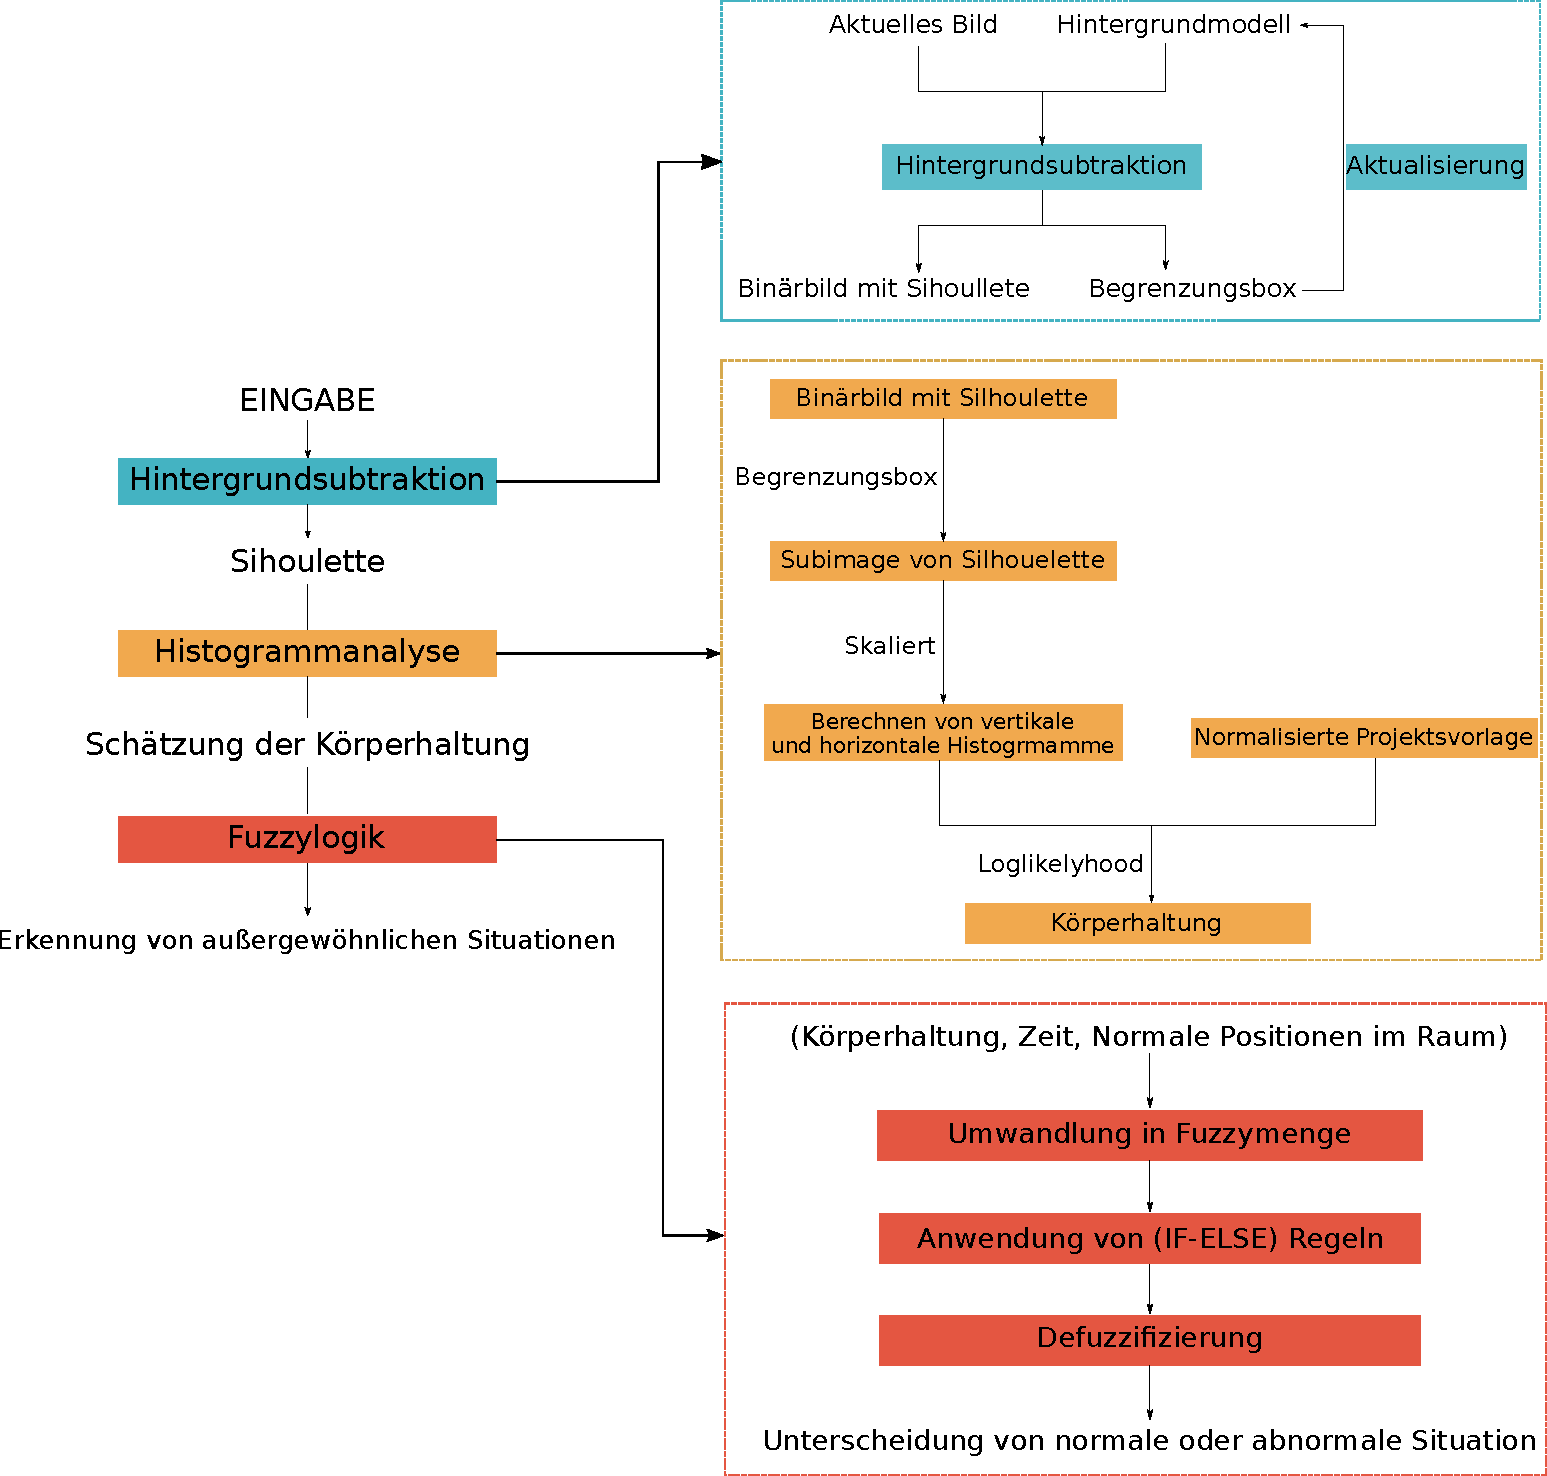
\includegraphics[width=1\textwidth]{fig/zusammenfassung.pdf}
	\caption{Zusammenfassung des Programmaufbaus. Die drei wichtige Meilenstein werden zum Verst�ndnis mit drei verschiedenen Farben dargestellt.}
	\label{fig:zusammenfassung}
\end{figure}
Um die Ergebnisse von dem Projekt zu evaluieren, wird jedes Testvideos w�hrend der Teste annotiert. Die Testergebnisse wurden mit unseren erwartetet Werte verglichen. Das Programm kann alle au�ergew�hnlichen Situationen richtig erkennen und die K�rperhaltung der Person mit einer Genauigkeit von �ber $70\%$ sch�tzen. Die Herausforderung der Arbeit besteht darin, die Verarbeitungszeit m�glichst gering zu halten. Bei einer durchschnittlichen Bearbeitungszeit von 109 Millisekunden pro Bild kann das Projekt als eine Echtzeitanwendung benutzt werden.\\

Es gibt in diesem Projekt noch ein paar Beschr�nkungen. Diese Anwendung erkennt eine Bewegung mit Hilfe von der Hintergrundsubtraktion, deswegen hat diese Anwendung auch das gleiche Problem wie bei der Hintergrundsubtraktion. Wenn es eine optische Tarnung in der Szene gibt, kann das Programm keine richtige Silhouette erkennen (siehe Abbildung \ref{fig:tarnung}). Es folgt auch eine falsche Sch�tzung der K�rperhaltung. Das zweite Problem ist: Wenn die Person weit weg von der Kamera ist, ergibt das Programm sich eine kleine Silhouette. Mit einer kleinen Silhouette kann die Anwendung die Sch�tzung der K�rperhaltung nicht richtig berechnen.\\

\begin{figure}[H]
	\centering
	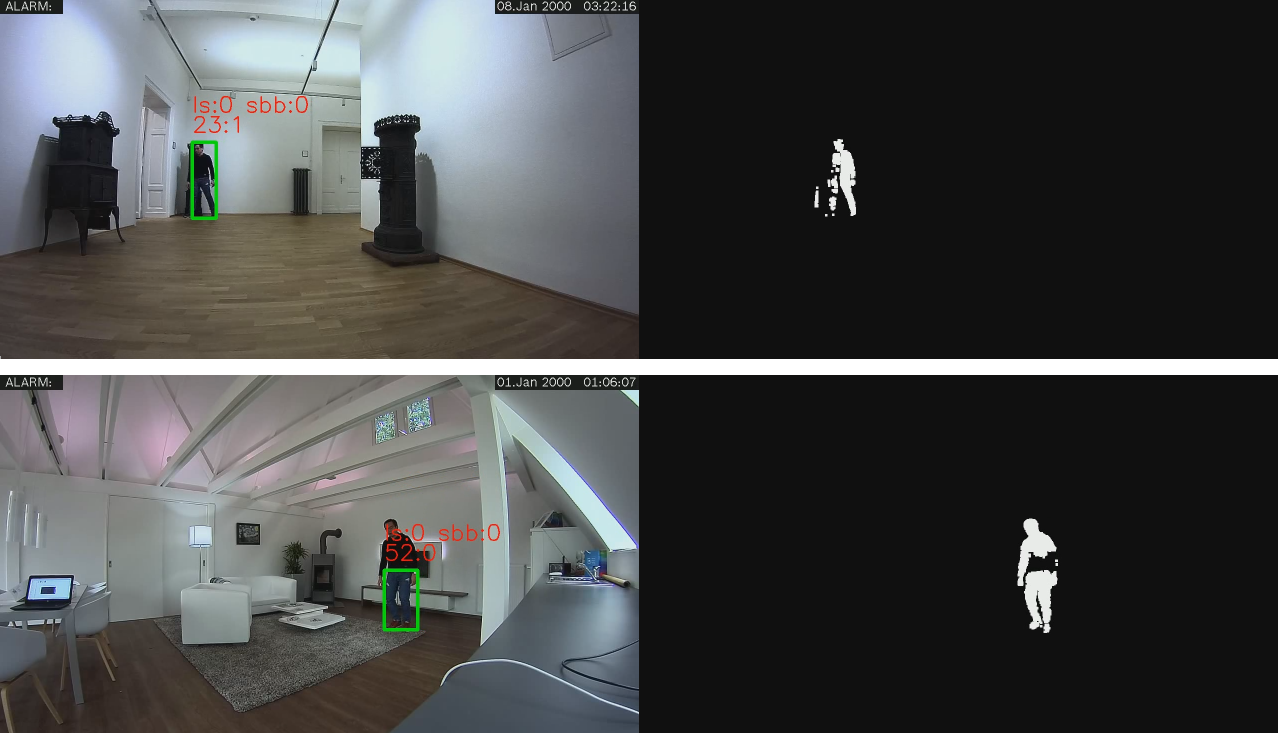
\includegraphics[width=1\textwidth]{fig/tarnung.png}
	\caption{Beispiele f�r die falsche Extraktion der Silhouette bei de Tarnungen. Auf den oberen Bildern ist die Testperson an einen schwarzen Kamin vorbei gegangen. In diesem Fall wurde die Person immer noch richtig erkannt. Auf dem unteren Bildern lief die Testperson an einen schwarzen Bildschirm vorbei. In diesem Fall wurde die Silhouette halbiert und es folgte eine falsche Erkennung der Testperson.}
	\label{fig:tarnung}
\end{figure}

Das Projekt hat viele Erweiterungspotenziale. Mir sind noch ein paar Ideen eingefallen, um das Programm noch umfangreicher zu machen.  Die erste Idee basiert auf der F�higkeit der Bewegungserkennung des Projektes. Die Kamera kann als ein Abwesenheitsmelder verwendet werden. Wenn es keine Bewegung in Haus in 24 Stunden gibt, dann wird eine Abwesenheitsmeldung ausgel�st oder ein Sicherheitsalarm wird automatisch angeschaltet. Meine zweite Idee ist eine Erweiterung des Projektes. Bis jetzt ist die Kamera noch nicht in die Smart Home App integriert. Wenn die Integration der Kamera mit der App realisiert wird, kann eine automatisch Lichtschaltung oder Heizungsschaltung sofort nach Erkennung einer Bewegung aktiviert werden. Die dritte Idee ist eine Verbesserung des Projektes. Heutzutage wird k�nstliche Intelligenz �berall verwendet. Mit Hilfe von neuronale Netz mit riesigem Datens�tzen kann die Sch�tzung der K�rperhaltung verbessert werden und damit wird die Qualit�t der Software auch deutlich erh�ht.